\documentclass{article}

% Language setting
% Replace `english' with e.g. `spanish' to change the document language
\usepackage[german]{babel}

% Set page size and margins
% Replace `letterpaper' with `a4paper' for UK/EU standard size
\usepackage[a4paper]{geometry}

% Useful packages
\usepackage{amsmath}
\usepackage{graphicx}
\usepackage[colorlinks=true, allcolors=blue]{hyperref}
\usepackage{float}
\usepackage{multicol}
\usepackage{xcolor}
\usepackage{subfiles} % Best loaded last in the preamble
\usepackage{tkz-euclide}

\setlength{\columnseprule}{0.5pt}
\def\columnseprulecolor{\color{blue}}


\title{Wirtschaft für Ingenieure}
\author{Asha Schwegler}

\begin{document}
\maketitle
\tableofcontents
\pagebreak

\section{Grundprinzipien der Betriebswirtschaft}
\subfile{subfiles/Grundprinzipien der Betriebswirtschaft}

<<<<<<< HEAD
\paragraph{Ökonomisches Prinzip:}
Spannungsverhältnis zwischen Unbegrenzte Bedürfnisse\\
und knappe Ressourcen.

\subsection{Gütereinteilung}
\paragraph{Güter werden aufgeteilt in:}

\begin{itemize}
\item Freie Güter
\item Wirtschaftliche Güter
\end{itemize}

\begin{figure}[H]
\centering
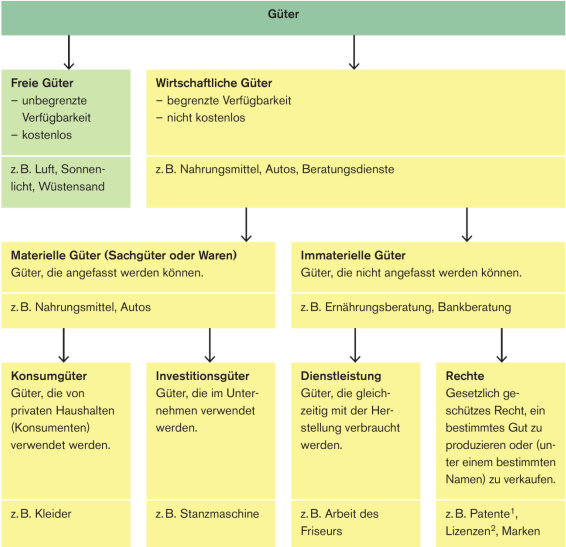
\includegraphics[width=0.3\textwidth]{Resources/Image/Guetereinteilung.png}
\caption{\label{fig:Guetereinteilung}Guetereinteilung.}
\end{figure}


\subsection{Markt}
Der Markt besteht aus Zusammenwirkung von Nachfrage und Angebot. \\
\subparagraph{Nachfrage:} Entsteht aus Bedarf, der wiederum aus Bedürfnisse entsteht.
\subparagraph{Angebot:} 
Entsteht aus der Herstellung


\subsection{Dreifache Unternehmensverantwortung}
\paragraph{Balance Akt zwischen:} 

\begin{itemize}
\item Gesamterhalt (Planet)
\item Selbsterhalt (Profit)
\item Miterhalt (People)
\end{itemize}

\begin{figure}[H]
\centering
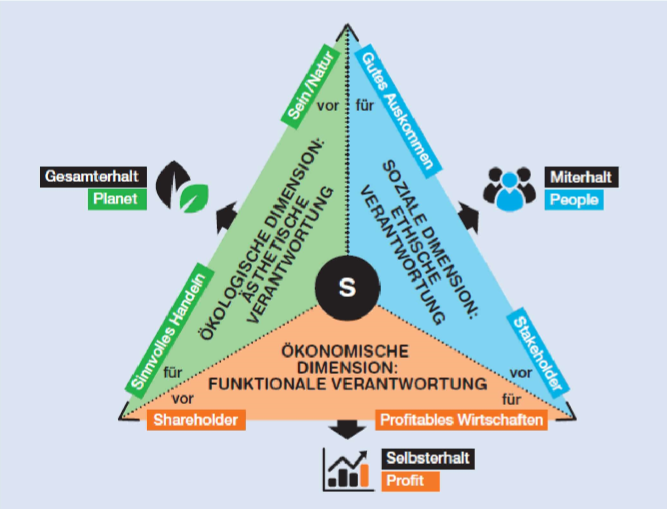
\includegraphics[width=0.3\textwidth]{Resources/Image/Dreifache Unternehmungsveratntwortung.png}
\caption{\label{fig:DreifacheUnternehmungsverantwortung}DreifacheUnternehmungsverantwortung.}
\end{figure}


\subsection{St. Galler Managementmodell}
\begin{figure}[H]
\centering
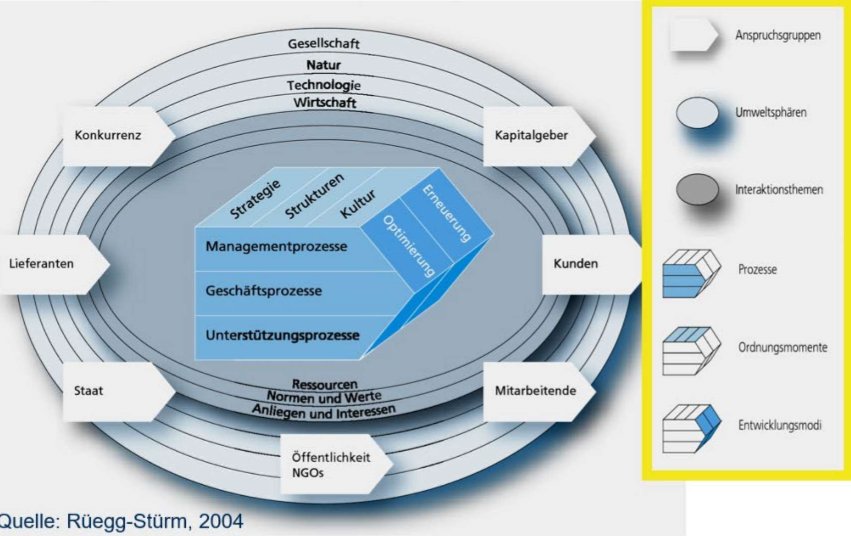
\includegraphics [width=0.3\textwidth]{Resources/Image/SGMM.png}
\caption{\label{fig:SGMM}SGMM.}
\end{figure}


\subsubsection{Umweltsphären}

\begin{tabular}{|l|l|}
\hline 
\rule[-1ex]{0pt}{2.5ex} \textbf{Umweltsphären} & \textbf{Beobachtungsbereiche} \\ 
\hline 
\rule[-1ex]{0pt}{2.5ex} Ökonomische Umwelt & Entwicklung Wirtschaft, Arbeitsmarkt, Teuerung, Wirtschaftsbeziehungen zum Ausland etc. \\ 
\hline 
\rule[-1ex]{0pt}{2.5ex} Technologische Umwelt & Produktionsverfahren, Materialien, Transport- und Kommunikationsmittel etc. \\ 
\hline 
\rule[-1ex]{0pt}{2.5ex} Soziale Umwelt & Politische und gesellschaftliche Trends, Wohlbefinden der einzelnen Menschen etc. \\ 
\hline 
\rule[-1ex]{0pt}{2.5ex} Ökologische Umwelt & Rohstoffe, Energie, Klima, Abfälle, etc. \\ 
\hline 
\end{tabular} 


\subsubsection{Anspruchsgruppen / Stakeholder}
\begin{enumerate}
\item Sind von der Tätitigkeit der Unternehmen betroffen. 
\item Haben Erwartungen und Ansprüche.
\end{enumerate}
 

\subparagraph{Machtausübung Primär:}
\begin{itemize}
\item faktische
\item vertragliche
\item gesetzliche
\item oder normative Grundlagen
\end{itemize}


\subparagraph{Sanktionsgrundlage Sekundär:}
\begin{itemize}
\item gesellschaftspolitische
\item witschaftsethische Konventionen
\end{itemize}

\begin{figure}[H]
\centering
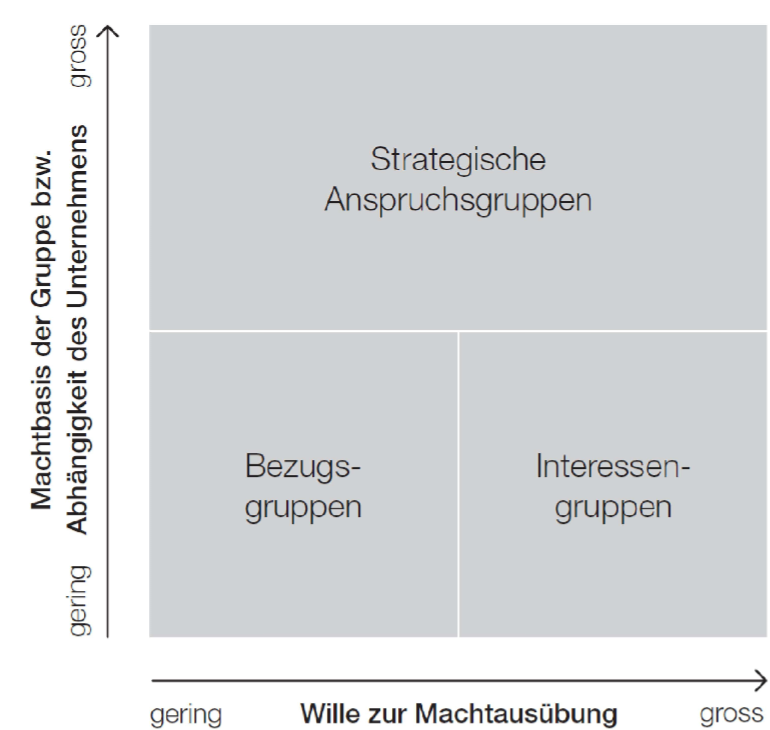
\includegraphics[width=0.3\textwidth]{Resources/Image/MachtausuebungStakeholder.png}
\caption{\label{fig:MachtausuebungStakeholder}MachtausuebungStakeholder.}
\end{figure}

\subsubsection{Interaktionsthemen}

\paragraph{Interaktionsthemenanalyse:}
\begin{enumerate}
\item Bestimmte Anspruchsgruppe
\item Anliegen und Interessen aufzeigen
\item Vorliegende Normen und Werte prüfen
\end{enumerate}

\paragraph{Ressourcen:}
\begin{enumerate}
\item Arbeit, Boden, Kapital, Wissen
\item Marke, Reputation, Image, Vertrauen
\end{enumerate}


\paragraph{Vorgehen:}

\subparagraph{1. Sachverhalt:}
\begin{itemize}
\item Welche Ressource des Unternehmens ist betroffen
\item In Welche Umweltsphäre spielt sich Sachverhalt ab
\end{itemize}

\subparagraph{2. Welche Anspruchsgruppe:}
\begin{itemize}
\item Anliegen / Ziele
\item Interessen
\item Normen (Gesetze und Regeln)
\item Werte
\end{itemize}

\subparagraph{3. Aus Unternehmenssicht:}
\begin{itemize}
\item Gefahren
\item Reaktionsmöglichkeiten
\end{itemize}

\begin{figure}[H]
\centering
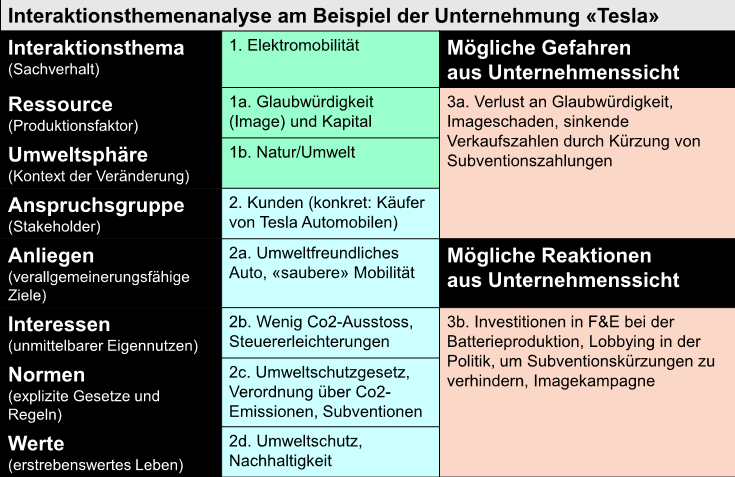
\includegraphics[width=0.3\textwidth]{Resources/Image/Interaktionsthemenanalyse.png}
\caption{\label{fig:Interaktionsthemenanalyse}Interaktionsthemenanalyse.}
\end{figure}
=======
\section{Strategie}
\subfile{subfiles/Strategie}
>>>>>>> d55c9eed1e1619c167e1f87d5f6539aa723e89dc

\pagebreak
\section{Marketing I}
\subfile{subfiles/Marketing1}


\section{Marketing II}
\subfile{subfiles/Marketing2}



\section{Erfolgsrechnung / Bilanz}
\subfile{subfiles/Erfolgsrechnung_Bilanz}

\section{Kostenrechnung}
\subfile{subfiles/Kostenrechnung}



\section{Kalkulation}
\subfile{subfiles/Kalkulation}


\section{Absatz-u.Produktionsplanung}
\subfile{subfiles/Absatz-u.Produktionsplanung}



\section{Personalmanagement}
\subfile{subfiles/Personalmanagement}



\section{Investitionsrechnung}
\subfile{subfiles/Investitionsrechnung}



\section{Realisation}
\subfile{subfiles/Realisation}
















































\end{document}